\section{System Design (Saroj)}
\label{sec:system_design}
\begin{itemize}
    \item KWS design
    \item Figure
\end{itemize}

%%% FIGURE: KWS ARCHITECTURE
%%% ------------------------
\begin{figure}[htbp]	
    %\centerline{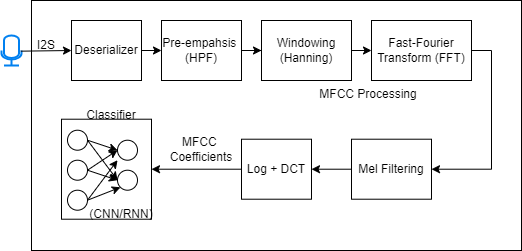
\includegraphics{figs/KWS-architecture.png}}
    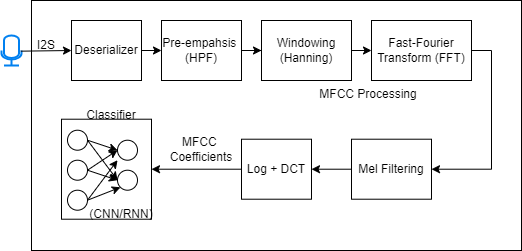
\includegraphics[width=0.45\textwidth]{figs/KWS-architecture.png}
    \caption{Implementation of a Keyword Spotter (KWS)}
    \label{fig:KWS_Arch}
\end{figure}

Acoustic audio analysis is widely used for important applications including heart monitoring, keyword spotting (KWS), and the preventative maintenance of heavy machinery. 
Among these methods, keyword spotting (KWS) plays a crucial role in various voice-activated smart assistants like Google Assistant and Amazon Alexa.
Fig.~\ref{fig:KWS_Arch} illustrates a well-known design of a digital KWS architecture. This design employs Mel frequency cepstral coefficients (MFCC) to derive spectral audio features from the input audio signal.
In this configuration, a digital microphone collects live data via an $I^2S$ serial interface. This stream of data is then converted to parallel bytes. The low-frequency portion of the signal is eliminated by applying a pre-emphasis filter (high-pass filter or HPF). The pre-emphasis filter is commonly realized by the following difference equation:
%%Equation: HPF
\begin{equation}
    y[n] = x[n] - \alpha~x[n-1] \label{eq:hpf}
\end{equation}
where, $\alpha$ is typically in the $0.9-1$ range.  
After the pre-emphasis filter is applied, the data is subjected to a window function (e.g., Hamming, Hanning, etc.) to prevent spectral leakage during the FFT operation.
After applying the window function, a fast Fourier transform (FFT) is performed on the signal to identify its frequency components. The linear frequency scale obtained from the FFT is known to be inadequate for replicating how the human ear perceives sound. Thus, the linear frequency spectrum is transformed into the Mel logarithmic scale, as given by:
%% Equation: Mel-log filter
\begin{equation}
    Mel(f) = 2595\cdot \log_{10}\left({1 + \frac{f}{700}}\right) \label{eq:mel-log}
\end{equation}
After applying the Mel log filter, the logarithm of the Mel frequency power is calculated, followed by a Discrete Cosine Transform (DCT) to derive the MFCC coefficients. These MFCC coefficients are then utilized to classify the voice signal using a classifier such as a convolutional neural network (CNN), recurrent neural network (RNN), long short term memory (LSTM), or other similar techniques.

Despite the architecture's popularity for KWS, the hardware implementation can differ greatly based on the application, which involves various trade-offs between power, area, and accuracy.
For this research, a \textit{smart microphone } application was examined in which the KWS is embedded directly into the microphone. This configuration allows it to recognize one or more keywords with moderate accuracy, while consuming minimum power while occupying a small area.
Now, each component is reviewed and determined on how to refine the design for this application. Digital microphones are generally built to record audio frequencies up to 22~kHz with a sample precision ranging from 12-16 bits. After capturing a keyword sample such as "Wakeup Neo", the data underwent low-pass filtering and reduction in precision using an open-source audio tool \textit{Audacity}. This procedure was progressively repeated until a noticeable effect was observed. Following multiple iterations, a 4 kHz bandwidth and 7-bit fixed-point precision were deemed adequate for the operation, resulting in significant area and power savings at the cost of minimal accuracy.
A similar optimization was performed for the HPF (Eq.~\ref{eq:hpf}) by selecting $\alpha=31/32=0.969$, which can be implemented using a basic \textit{shift-and-add} operation rather than a hardware multiplier. 
A hanning window was selected for the windowing function, and the coefficients were implemented using exclusively single shift operations, resulting in substantial hardware savings with a minor increase in spectral leakage. 

%%% ------------------------
%%% RTL-to-GDS Design Flow
%%% ------------------------
\subsection{RTL-to-GDS Design Flow}

%%% FIGURE: RTL-TO-GDS Desing Flow 
%%% ------------------------
\begin{figure}[htbp]
	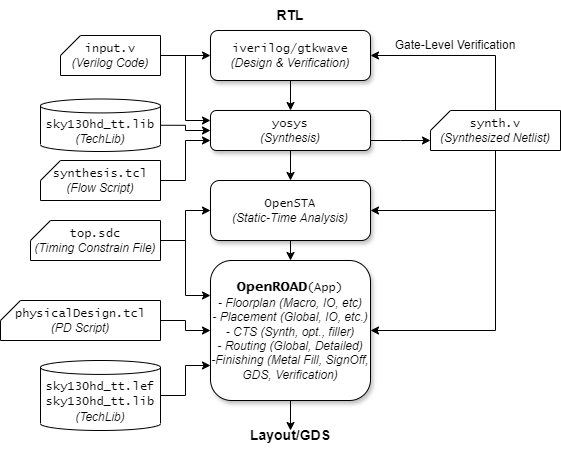
\includegraphics[width=0.45\textwidth]{figs/rtl2gds-toolchain.png}
	\caption{RTL-to-GDS design flow using open-source tools.}
	\label{fig:RTL-to-GDS}
\end{figure}

